\documentclass{IEEEtran}
\usepackage{amssymb}
%\usepackage[francais]{babel}
%\usepackage[utf8]{inputenc}
\usepackage{amsmath}
\usepackage{amscd}
\usepackage{hyperref}
\usepackage{verbatim}
\usepackage{subfigure}
\usepackage{tikz}
\usepackage{proof}
\usepackage{alltt}
\usepackage{color}
\usepackage{xspace}
\usepackage{tikz,ifthen}
\usepackage{fancybox}
\usepackage{wrapfig}
\usepackage{multirow}
\usepackage{listings}
\usepackage{rotating}
\usepackage{xcolor,colortbl}
\usepackage{epstopdf}
\usepackage[textsize=small,colorinlistoftodos]{todonotes}
\pagestyle{plain}
%
\usepackage{makeidx}  % allows for indexgeneration
\usepackage{algpseudocode}
\usepackage{algorithm}


\newcommand{\ft}[1]{{\small\textsf{#1}}}
\newcommand{\uppaal}{\textsc{Uppaal}\xspace}
\newcommand{\uppaalsmc}{\textsc{Uppaal SMC}\xspace}
\newcommand{\R}{\mathbb{R}_{\ge 0}}

\newcommand{\CR}{\emph{WCRA}_c^r}
\newcommand{\CW}{\emph{WCRA}_c^w}
\newcommand{\MR}{\emph{WCRA}_m^r}
\newcommand{\MW}{\emph{WCRA}_m^w}

\newtheorem{definition}{Definition}
%\newtheorem{theorem}{Theorem}
%\newtheorem{property}{Property}



\IEEEoverridecommandlockouts


\title{Performance Driven Scheduling of Multicore Time-critical Systems \thanks{This work has been supported by the NFFP6 Project.}}


\author{
\IEEEauthorblockN{Jalil Boudjadar, Jin Hyun Kim, Simin Nadjm-Tehrani} \\
\IEEEauthorblockA{Department of Computer and Information Science \\ Link\"oping University, Sweden} 
}


\begin{document}
\maketitle


\begin{abstract}
Multicore platforms are getting widely used in the deployment of embedded systems due to their computing capacity. Memory interference represents a challenge in leveraging the performance of multicore platforms and may lead to drastic degradations of the platform performance, in particular for memory-intensive systems. This paper explores performance-driven schedulability of  multicore systems by evaluating the performance when changing some design parameters (scheduling policies). The model-based framework we build enables to analyze the performance of multicore time-critical systems running core-centric and memory-centric scheduling policies. The system architecture we consider consists of a set of cores having each a local cache and sharing the cache level L2 and DRAM. The metrics we use to compare the performance achieved by different configurations of a system are: 1) cores utilization; and 2) the maximum delay per access request to shared cache and DRAM. Our framework, realized using Uppaal, can be viewed as an engineering tool, to be used during design stages, to identify the scheduling policies achieving  better performance for a given system while maintaining the system schedulability. As a proof of concept, we analyze 2 different cases studies and compare the outcomes.
\end{abstract}



\section{Introduction}
\label{sec:introduction}


Today's embedded systems demand increasing computing power to accommodate the growing software functionality. 
Multicore platforms are finding their way into Automotive and avionic areas where they are a target to deploy safety-critical applications. In avionic systems, an ultimate goal of using multicore platforms is to leverage the computing capabilities, reduce the weight of on-board computing equipment and lower the energy consumption. Such multicore avionic systems are usually built by integrating different subsystems, potentially provided by different vendors, to enable incremental Design and Certification (iD\&C) \cite{iDC}, recommended by the standard Integrated Modular Avionics (IMA) architecture \cite{ima}. 
%
However, due to the safety guarantees and hard critical requirements performance can be sacrificed, up to a certain degradation level, if the safety and reliability are in peril. Performance is then considered as a second class property that is aimed to be as high as the system safety permits.  

In contrast to the classical federated architecture, IMA supports functions related to different subsystems to share the same computing platform with an efficient use of the hardware. Such a support is implemented using partitioning, where different partitions running on different cores compete for the access to a set of shared resources, such as shared memories and buses. 
%
%Multicore designers have achieved much progress on improvement of memory-dependent performance in caching systems and shared memories in general. 
However, having applications running simultaneously and requesting the access to the shared memories concurrently leads to interference. The non predictability resulting from interference at any shared memory level may lead to violation of the timing properties in safety-critical real-time systems. Moreover, the interference on shared memories leads cores to stall, in particular for read access requests, so that the performance is affected as well. Hence, bounding memory interference is a key factor to guarantee schedulability and improve performance \cite{Kim14}.

Strong efforts have been devoted to the analysis of safety and predictability of multicore systems \cite{Lisper14,Nowotsch14,Andersson2010,Chatto2012,5753612}, however less studies focusing on the compensation of performance while maintaining the timing predictability guarantees have been achieved \cite{DBLP:journals/corr/TeodoroKAKFS15,6280389,Sarkar:2011:PTM:1967677.1967696,10.1109/MS.2005.102,Subramanian13}. When designing a software system, there is a potential margin where a drift configuration, obtained by slightly tweaking the original system e.g. by assigning tasks differently to cores or using much optimal scheduling policies, can functionally behave in the same way while achieving better performance and satisfying the predictability requirements \cite{SHARMA2014544,Sarkar:2011:PTM:1967677.1967696,5753612}.   

This paper represents a performance-driven schedulability framework for multicore systems. Such a model-based framework  
enables to analyze and improve the performance of multicore systems when changing cores scheduling policies (design parameters), while maintaining systems schedulable so that system configurations achieving better performance can be identified and planned for deployment. We adopt the Asymmetric Multi-Processing (AMP) \cite{Huyck12} avionic scheduling architecture, where partitions are statically allocated to specific cores. Moreover, the processor scheduling alternatives we consider are memory-centric and core-centric. The platform architecture consists of a set of cores having each a local cache, and sharing the cache level L2 and DRAM. We use the cache coloring policy \cite{Hyoseung13} to arbitrate concurrent access requests to the shared cache at level 2 (L2). In addition, we adopt the policy {First Ready-First Come First Serve (FR-FCFS)} \cite{Rixner2000,Kim14} commonly used by modern COTS-based memory controllers to schedule the DRAM access requests.   
%
The application model is given by a set of periodic task sets, each of which is assigned to a given core and scheduled using either memory-centric or core-centric policies. Moreover, application tasks have explicit read and write access numbers for shared caches and DRAM. We distinguish between read and write access requests to shared memories as read actions are blocking for cores, while write actions are not blocking and can be performed using dedicated buffers.

The performance metrics we consider are the \textit{utilization of cores} and \textit{maximum delay per access request} to shared memories (L2 cache and DRAM). We provide rigorous schedulability analysis using symbolic model checking, while performance metrics are measured using statistical model checking. %Our framework is realized as an engineering toolbox to be used at design stage to identify the scheduling policy leading to higher performance while maintaining the schedulability property.


 

%This paper introduces a formal framework, using Uppaal \cite{Uppaal}, for the schedulability analysis and estimation of interference-sensitive WCET (isWCET) of multicore systems. The framework includes both local and shared caches as well as a shared DRAM. We use the cache coloring policy \cite{Hyoseung13} to arbitrate concurrent access requests to the shared cache at level 2 (L2). In addition, we adopt the policy {First Ready-First Come First Serve (FR-FCFS)} \cite{Rixner2000,Kim14} commonly used by modern COTS-based memory controllers to schedule the DRAM access requests. The schedulability analysis is rigorously performed using the symbolic model checker of Uppaal, while the isWCET is computed using the Uppaal statistical model checker. By statistical we mean  simulating different executions but not exploring the whole state space. The analysis is performed based on the WCET of individual tasks, how many times each task needs to read from and write to DRAM and L2 cache.%, as well as page coloring and FR-FCFS as scheduling policies.  



%The rest of the paper is organized as follows: Section~\ref{sec:relatedwork} reviews the related work. Section~\ref{sec:background} describes the necessary background. Section~\ref{sec:methodology} provides an overview of our work. Section~\ref{sec:modeling} presents Uppaal templates included in our framework, whereas Section~\ref{sec:analysis} describes schedulability, isWCET analysis and method for potential reallocation of tasks. %as well as migration of tasks. In Section~\ref{sec:casestudy}, a small case study is presented to show preliminary evidence of the feasibility and efficacy of the framework. Finally, Section~\ref{sec:conclusion} concludes the paper.  



\section{Related Work}
\label{sec:relatedwork}

\cite{10.1109/MS.2005.102} performance analysis techniques 

\cite{Rakhee2014} performance measurement of multicore systems

\cite{DBLP:journals/corr/TeodoroKAKFS15} performance analysis of multicore systems

\cite{5762713} evaluation and optimization of the performance

\cite{Subramanian13} Providing performance predictability and improving memory interference 

\cite{SHARMA2014544} The tool also provides the possibility of implementing different scheduling and mapping algorithms for multi-core process systems and evaluating the performance when changing various design parameters.


%Analyzing the schedulability of an application while considering an abstraction of the execution platform leads necessarily to underestimate the system requirements (workload) in terms of resources. This may cause serious deficits when deploying the system on a concrete platform. 

The analysis of multicore real-time systems has attracted a lot of attention recently. 

In this work, we combine the analysis processes so that for a given platform we check whether the application tasks will be schedulable or not, given the task WCETs estimated in isolation. Our framework provides also the ability to calculate the isWCET and a method for reallocation of tasks to cores upon non-schedulability. 
 %In case a system is not schedulable, given the actual interference we analyze the cores utilization and recommend a change in tasks allocation among cores so that a new configuration could be schedulabe. 
The novelty of our modeling approach is the inclusion of cache coloring policy \cite{Hyoseung13} to arbitrate concurrent access requests to the shared cache, FR-FCFS policy \cite{Rixner2000,Nesbit2006,Kim14} commonly used by modern memory controllers to schedule the DRAM accesses, while distinguishing between read and write requests. 

%Given a multicore execution platform, including processing units, local caches and a shared memory, we formally analyze the system schedulability. Moreover, our framework can easily be used to estimate the concrete execution time, including cache access and blobking/access time to the shared memory, of the application tasks.    



\section{Background}
\label{sec:background}
%Before diving into the description of our contributions, we introduce the fundamental background of our work.

In multicore settings, assessement of the execution time and memory interference has become a challenge because the number of possible interleavings increases exponentially with the number of processes, number of cores and number of shared resources \cite{Chatto2012}. In practice, concurrent programs may have astronomical numbers of legal interleavings which makes the interleaving analysis not feasible. An alternative is to reuse the knowledge acquired from the single core analysis and just focus on the interference resulting from the access to shared memories. This section introduces benchmarking, as a technique to measure WCET and WCRA, as well as the fundamental background of our work.

\begin{figure}[ht!]
\centering
\caption{Simplified multicore system architecture.}
\label{fig:architecture}
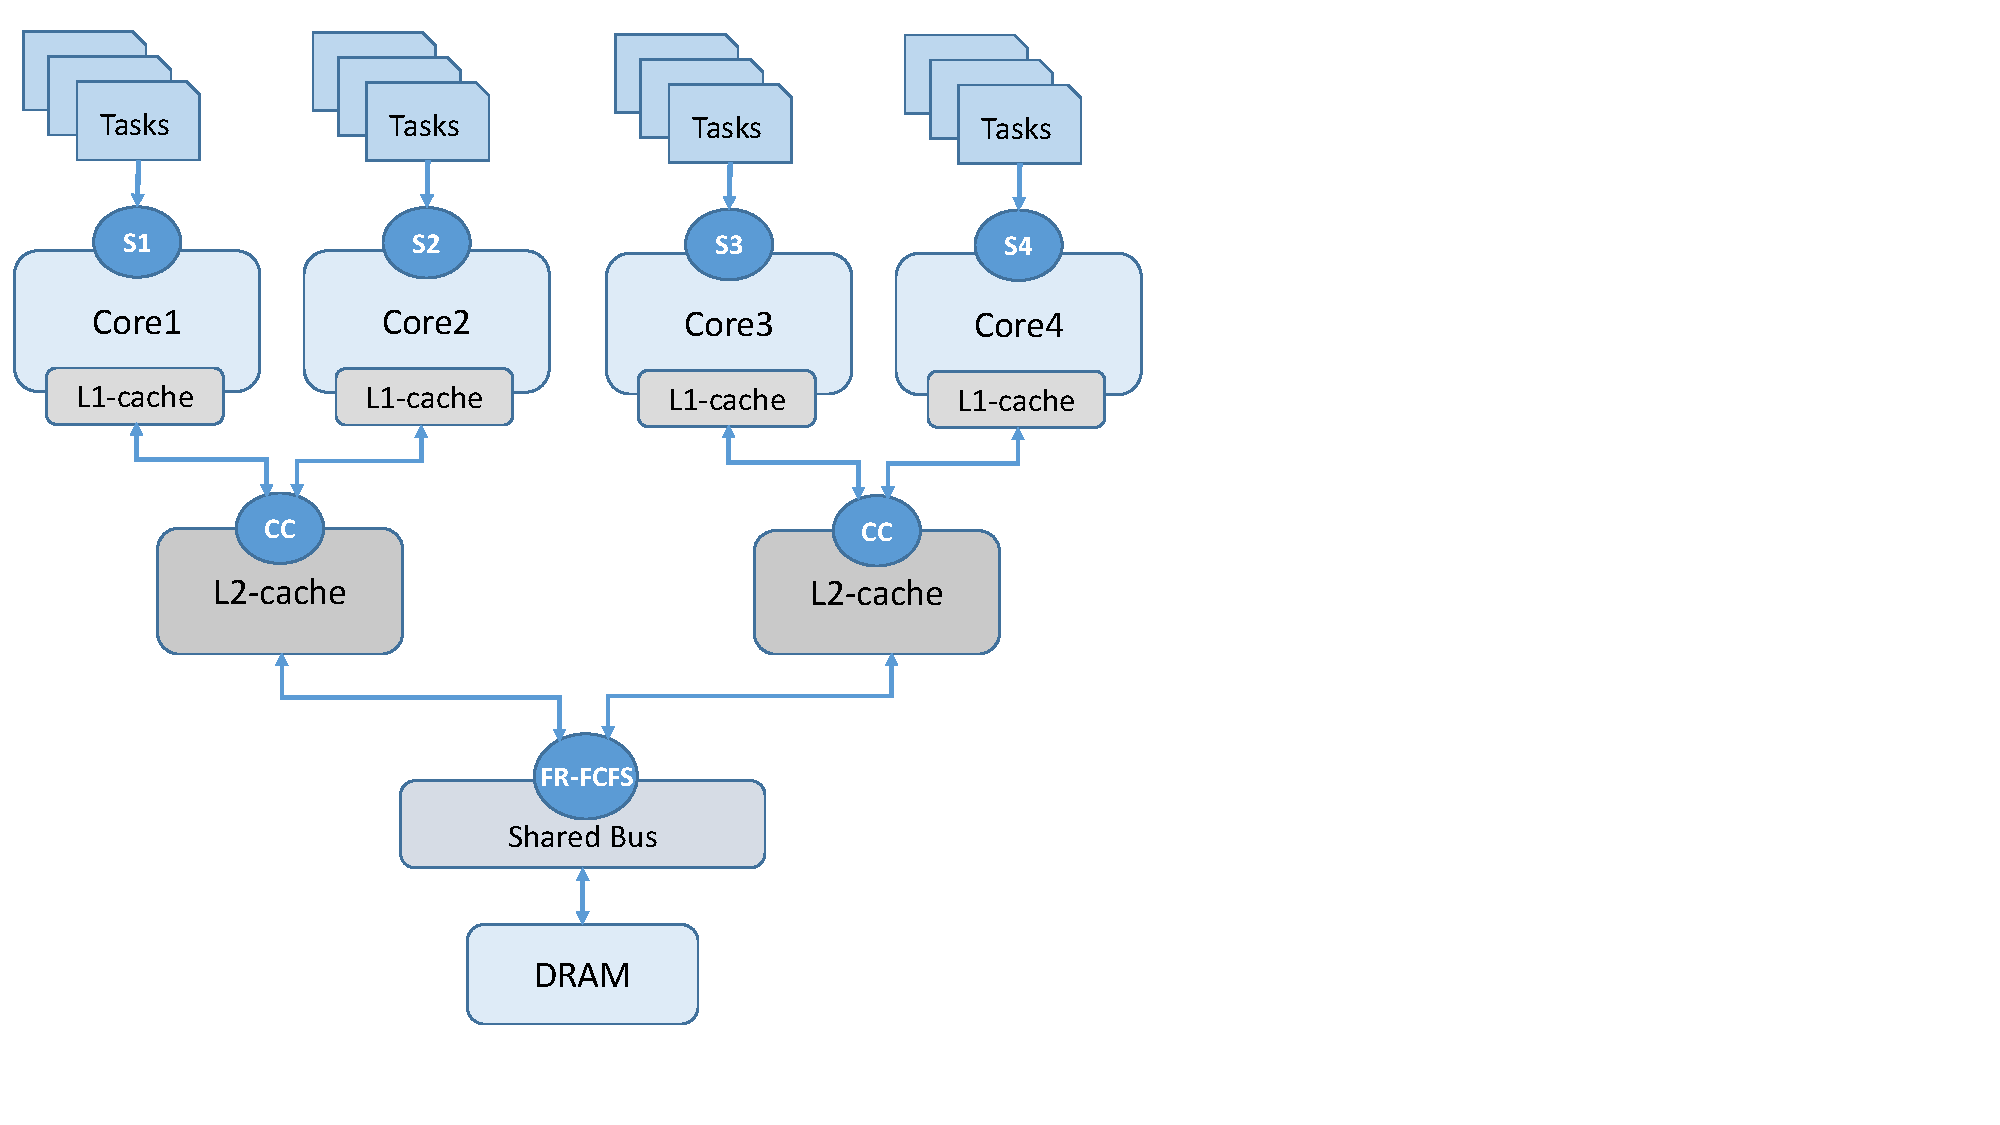
\includegraphics[scale=0.45]{architecture.pdf}
\end{figure}

The overall system architecture we consider in this paper is depicted in Fig.~\ref{fig:architecture}, where $cc$ is the cache coloring policy and $s_i$ are CPU scheduling policies.

\subsection{Systems Benchmarking} 
\label{sec:methodology}
Throughout this section we describe how the inputs required by our model-based framework are obtained form an actual system, in particular WCETs and WCRAs. In software engineering, benchmarking \cite{Benchmarking} aims at measuring a set of execution attributes and performance characteristics, e.g. WCET, of a given software system. %The user has to run the application to be benchmarked on the target platform to determine for example the execution time of each process. 
The output of a system benchmarking (shortly known by benchmark) will be used to reconstruct a behavioral model of the system,  which can be used in turn for simulation and analysis purposes. Benchmarking is known as an expensive operation that involves several iterative rounds in order to reach conclusive decisions. %In this context, we are interested in how WCET and WCRA are derived from a concrete multicore software system. 
Roughly speaking, flow analysis and profiling are the most commonly used techniques to measure the WCET and WCRA of application tasks.  

Flow analysis \cite{Tan2009,Chatto2012} is a technique to estimate the WCET of a program. It consists of simulating, or concretely running, a program in isolation and measuring the time spent. Technically, static analysis tools use symbolic execution engines to identify potential execution paths without necessarily having to run the program. Such representations can be structured in terms of control flow graph (CFG). %Similarly to compilers, a static analysis tool parses a source code of a program and converts it to an intermediate representation where each state could be a class of different program configurations. 
WCET is then the time spent when executing the longest path of the CFG. Static analysis has been practiced for the analysis of software systems via different analysis tools, e.g. {SWEET} \cite{Tan2009}. 
%The depth of the model determines the effectiveness of the tool. That depth is based on how much knowledge of program behaviour is built in, how much of the program it can take into account at once and how accurately it reflects actual program behaviour. 

%Conventionally, task periods and deadlines (potentially also priority and criticality levels) are identifiable during the requirements analysis.

System profiling \cite{Yun2012,Kim14} is a measurement-based approach to estimate how many times a process accesses  shared memories. The system being analyzed is run for a sufficient number of times, each of which for a long enough duration enabling the execution of most of the system functions (code). The analysis focuses on each process individually, so that for each run we track how many times a process accesses a given shared memory. However, due to technology limitations, the measurements can be performed at core level only, so that the obtained access number of a given core corresponds to the set of processes running on top of it. In order to obtain the memory access number for each process, one needs to run each process individually on one core during the analysis, so that the access number obtained corresponds to the process being run. The number of accesses for each core can be obtained using Performance Monitor Counters (PMCs) \cite{Yun2012}, equipping certain multicore platforms. %Such a number is commonly called \textit{Worst Case Resource Access} (WCRA) \cite{Nowotsch14}. 

In literature \cite{Kim14,Yun2012}, profiling and static analysis techniques are not completely differentiated. Both techniques can be used to measure WCET and WCRA.
  

%Once the attributes of system tasks are determined, one can apply rigourous schedulability analysis tools suing either analytic approaches \cite{***} or model-based enginnering approaches \cite{***}.   
 
\subsection{Core-centric Scheduling}
To leverage the processing performance of a computing system, a processing unit (core in our context) can be assigned more than one task, however only one task can execute effectively at any point in time. The arbitration between the different tasks execution is performed according to a scheduling policy. 

Basically, a scheduling policy determines, at any point in time, which task from the ready queue must execute first and whether a given task should be preempted by another. Such a ready queue can be either local for a given core (Local scheduling) or common for a set of cores (Global Scheduling). The most commonly used scheduling algorithms are {Earliest Deadline First} (EDF), {Fixed Priority Scheduling} (FPS) and {Rate Monotonic} (RM). The key factor in selecting a task from the ready queue can be assigned to the priority, remaining execution time, etc. 
 
In our setting, we adopt FIFO, FPS and EDF as scheduling policies for the individual cores.  %Classic static (cyclic) scheduling used in aerospace contexts can also be coded as a policy if needed. 

\subsection{Memory-centric Scheduling}

%In multicore settings, where different applications running concurrently on different cores compete for the combination of local cache misses and interference delay for accessing a shared  memory can be large and highly variable depending on the platform architecture and the number of parallel access requests. 

With the goal to reduce memory interference in multicore systems, a recent alternative to schedule memory-intensive application tasks is the use of a memory-centric policy \cite{Yao2015,Yao2012}. Tasks assigned to the same core are sorted in the ready queue according to a decreasing order of their WCRA (numbers of memory accesses). 

We distinguish between the access numbers to L2 and DRAM, when comparing 2 tasks we prioritize first the task having more DRAM access requests as DRAM access is more expensive than accessing shared cache L2. If both tasks have the same DRAM access number of requests we refer then to their L2 access number where task having higher number is scheduled first.


 

\subsection{Shared Memory Access Scheduling}
In order to enhance the processing performance of multicore platforms, some of modern multicore processors \footnote{E.g. {Intel Core i7, AMD FX, ARM Cortex and FreeScale QorIQ} processors.} consider a shared cache level (L2-cache) besides to private caches (L1-cache). The primary goal of sharing a cache between different cores is to reduce the access requests to the main memory DRAM  %further, and by that shorten the DRAM interference time since the interference time is strongly correlated to the number of access requests
 \cite{Nowotsch14}. %On the other hand, uncontrolled sharing of cache can lead to a degradation of performance and lack of predictability where starvation can arise. 


Cache coloring policy \cite{Hyoseung13,Ye2014} is an algorithm to control the access to the shared cache level L2. It has been introduced to aid performance optimization where physical memory pages are mapped to cache pages, in contrast with old caching systems where virtual memory is mapped to the cache. This entails avoiding the clearance of cache pages on each context switch. 
During execution, the algorithm frees the old pages as necessary in order to make space for currently scheduled applications (recoloring). The coloring algorithm sorts the concurrent access requests according to their release times.  
 
%Another alternative to schedule accesses to DRAM, in presence of a three-dimensional structure (bank, row and column), is the {Hit-First} policy. The Hit-First algorithm schedules row buffer hits before misses to reduce the average memory access latency and to improve bandwidth utilization \cite{Hong99,Rixner2000}. This is due to the fact that requests hitting in the row buffer have shorter latency than a row buffer miss.

To maximize data throughput and minimize the DRAM latency, DRAM controllers in modern COTS-based systems use {First Ready-First Come First Serve} (FR-FCFS) as a DRAM policy \cite{Rixner2000,Kim14}. FR-FCFS considers a detailed DRAM architecture structured in terms of banks, rows and columns. %The DRAM scheduler can be viewed as a 2-level filter: bank level and bus level. 
The access requests can target different banks separately, where they will be queued in the corresponding bank queue with a special preference to read requests since they cause the processor to stall. % while write requests can normally be performed using write buffers. 
Access requests will be sorted at each bank queue first according to their readiness. Thereafter, the candidates selected from banks level will be further sorted at bus level where the earliest request gains access, i.e. the first request showing up at bus level among the requests being selected by bank schedulers. If no request hits the row-buffer, older requests are prioritized over younger ones.  

In our framework, we do not consider the detailed internal architecture and size of DRAM and shared cache. We focus rather on measuring the delays caused by the concurrent accesses. The reason behind this is that the impact of these characteristics on the
interference is already captured when performing the static analysis and identifying the WCRAs. Hence, estimating the optimal cache size for each application and cache recoloring are beyond the scope of this paper.


\subsection{Statistical Model Checking}
We are using \uppaalsmc \cite{SMC} to perform a formalized statistical simulation of our models, known as Statistical Model Checking (SMC). SMC enables quantitative performance measurements instead of the Boolean (true, false) evaluation that symbolic model checking techniques provide.    
We can summarize the main features of \uppaalsmc in the following:
\begin{itemize}
\item Stopwatches \cite{DBLP:conf/concur/CassezL00} are clocks that can be stopped and resumed without a reset. They are very practical to measure the execution time of preemptive tasks.
\item Simulation and estimation of the expected minimum or maximum value of expressions over a set of runs, \texttt{E[bound](min:expr)} and \texttt{E[bound](max:expr)}, for a given simulation time and/or number of runs specified by \texttt{bound}. 
\item Probability evaluation \texttt{Pr[bound] (P)} for a property \texttt{P} to be satisfied within a given simulation time and/or number of runs specified by \texttt{bound}. \texttt{P} is specified using either LTL or tMITL logic. 
\end{itemize}

Statistical model checking does not provide complete certainty that a property is satisfied, but only verifies it up to a specific confidence level \cite{DBLP:conf/formats/DavidLLMPVW11}, given as an analysis parameter.


\section{Performance Metrics}
This section defines the performance metrics we have chosen as a basis to compare memory-centric and processor-centric scheduling policies. We analyze the performance on a set of independent runs $\emph{Runs}=\{\pi_1, \pi_2, \ldots\}$, randomly generated from a standard cylinder construction according to a probabilistic semantics \cite{DBLP:conf/formats/DavidLLMPVW11}. A run $\pi$ of a system $S$ is an infinite sequence:
\[ \pi = s_0 (t_0,e_0) s_1 (t_1,e_1) \ldots s_n (t_n,e_n) \ldots \]
\noindent
where each states $s_i$ gives information about a system configuration including the state of each  task (e.g.  idle,  ready,  running,   blocked)  and  resource (e.g. idle,  occupied) at stage  $i$; $s_0$ is the initial state. Each $e_i$ indicates an event (triggering,  queued or completing) signifying a transition from state $s_i$ to $s_{i+1}$. Timestamp $t_0$ indicates the time from system initiation until event $e_0$. Every subsequent timestamp $t_i$ (with $i \geq 1$) indicates the separation between events $e_{i-1}$ and $e_i$.

Moreover, for a given run $\pi$ we introduce the following the obvious predicates: 
\begin{itemize}
\item $\emph{InUse}_{\pi}^s(C)\in\mathbb{N}$ states whether the core $C$ is in use in state $s$ of $\pi$ or not. In fact, a core is in use if it is either effectively executing a workload or stalling due read access requests to L2 and DRAM.   
\item $\emph{Issued}_{\pi}^C(\emph{req})$ indicates at which state of $\pi$ the access request \emph{req} performed by core $C$ has been issued.
\item $\emph{Granted}_{\pi}^C(\emph{req})$ states the earliest state at which the request \emph{req} performed by core $C$ has been granted.
\end{itemize}
 
\begin{definition}[Core utilization]
The utilization $\emph{U}_{\pi}^{{\cal L}}(C)$ of a core $C$ for a given run ${\pi}$ up to the time bound (simulation length) {\cal L} is given by the following:\\ 
%\vspace{-2mm}
\begin{footnotesize}
\[
\emph{U}_{\pi}^{{\cal L}}(C) = (\limsup_{t\rightarrow {\cal L}} \frac{\sum\limits_{t_{i+1}\le {\cal L}}((t_{i+1}-t_i)\times \emph{InUse}_{\pi}^{s_{i+1}}(C))
}{{\cal L}}) \times 100
\]
\end{footnotesize}
%\vspace{-3mm}
\end{definition}

The average utilization of a core $C$ over the set of runs $\emph{Runs}$, analyzed for the same time interval length {\cal L},  will be the sum of the individual runs utilization on the number of runs:
\[ \emph{U}_{\emph{Runs}}^{{\cal L}}(C)=\frac{\sum\limits_{j=1}^{j= \mid\emph{Runs}\mid} \emph{U}_{\pi_j}^{{\cal L}}(C)}{\mid\emph{Runs}\mid}
\]

\begin{definition}[Interference of access requests]
We define the interference delay of a request \emph{req} performed by a core $C$ in a run $\pi$ as follows: $\emph{ReqDelay}_{\pi}^C(req)=\emph{Granted}_{\pi}^C(\emph{req})-\emph{Issued}_{\pi}^C(\emph{req})$. 

In similar way, we define the maximum delay of the requests $\emph{Req}_C$ performed by a core $C$ over a run $\pi$ by: 
\[\emph{ReqDelay}_{\pi}^C= \max(\emph{ReqDelay}_{\pi}^C(req\mid req\in Req_C))\]
\end{definition}

The average of maximum interference delays performed by a core $C$ over the set of runs \emph{Runs} can be calculated as follows: 
\[ \emph{ReqDelay}_{\emph{Runs}}^C=\frac{\sum\limits_{j=1}^{j= \mid\emph{Runs}\mid} \emph{ReqDelay}_{\pi_j}^C}
{\mid\emph{Runs}\mid}\]

As access requests to L2 and to DRAM do not have the same impact on the interference, later on we distinguish between $\emph{L2\_ReqDelay}_{\emph{Runs}}^C$ and $\emph{DRAM\_ReqDelay}_{\emph{Runs}}^C$ as the interference delays of a given core $C$ to access L2 and DRAM respectively. 

\section{System Model Description}
\label{sec:modeling}
%Basically, an embedded system is given by an application mapped to a platform. The application is a parallel composition of tasks.
The platform we consider consists of a set of cores (processing elements), one shared cache level and a shared DRAM. %and mechanisms to share and control the access to the platform resources like processor schedulers and DRAM connectors. 
The application is given by a set of tasks mapped to different cores. Mainly, application tasks are characterized by their computation times WCET (measured when each task runs in isolation), and the worst case resource access numbers (WCRA) \cite{Nowotsch14} to DRAM and shared cache L2 for both read and write actions. Access requests to shared memory are non-deterministically spread out along the task execution. The reason behind that is that tasks execution, and thereby the issue time of data requests, may vary from one period to another following the changes in the computation environment. 

We use ${\cal T}$ for the set of tasks and ${\cal C}$ for the set of cores. The assumptions about the systems we consider are the following: 
%
\begin{itemize}
\item Tasks are periodic and non-preemptible during CPU use. 
\item Tasks assigned to the same core are arbitrated using a local scheduler. 
\item We consider a local cache (L1) for each core, only one shared cache (L2) and one DRAM for all cores.
%\item We abstract each local cache using a number stating the time for fetching data from it. %The number of local cache misses corresponds to the WCRA number to L2.  
%\item Tasks are assigned statically to PE so that a task always executes on the same core. Later on, but our framework can easily be extended with dynamic assignment to incorporate migration and workload balance.
\end{itemize}

\subsection{Application Model}
An application $AP=\{T_1,..,T_n\}$ is a set of tasks each of which describes the execution model of an individual process. The process behavior is abstracted at task level using WCET and WCRA for both shared cache and DRAM. WCET is the pure execution time, calculated in isolation when a task runs alone on a single core. Regarding data fetching, we consider 2 attributes $\emph{WCRA}_c$ and $\emph{WCRA}_m$ where: $\emph{WCRA}_c$ corresponds to the maximum number of successful accesses (hits) to the shared cache L2; $\emph{WCRA}_m$ is the number of DRAM accesses (corresponds to L2 miss) performed by a given process. Moreover, in order to distinguish between read and write accesses to each shared memory, we denote each of the attributes with $r$ for read and $w$ for write, i.e. $\CR, \CW, \MR$ and $\MW$. This is because read requests make the core stalling (strong impact on isWCET) while write requests do not as they can be performed using dedicated buffers. Such patterns are identifiable using abstract interpretation \cite{Wang2010} and program/cache analysis \cite{Ferdinand1999}, e.g. the PAG tool \cite{PAG}, on a given platform architecture. %As stated earlier, the duration for fetching data from a shared memory varies because of the interference.    

An access request to a shared memory is given by a $\emph{pattern}\in \{L2, DRAM\}$ stating to which memory the access hits and an attribute $RW$ indicates whether it is a read ($r$) or write ($w$) action. Moreover, as we need to keep track of when the requests are issued, so that FR-FCFS algorithm determines the priorities of requests targeting DRAM, we use \emph{issueTime}. 
In fact, \emph{issueTime} is initially empty and will be initialized by a core when the access request is triggered. Accordingly, an access request is formally given by $\emph{req}=\langle \emph{pattern}, RW, \emph{issueTime}\rangle$. 
$\CR$ and $\CW$, respectively $\MR$ and $\MW$, of a given task are then the numbers of read and write accesses to L2, respectively DRAM.

\begin{definition}[Task structure] A task $T$ is given by $\small{\langle \emph{Prd}, \emph{Offset}, \emph{WCET}, \CR, \CW, \MR,\MW, \emph{Dln}, \emph{Pri}\rangle}$ where $\emph{Prd}$ is the task period, $\emph{Offset}$ is the periodic offset, $\emph{WCET}$ is the pure execution time, $\emph{Dln}$ is the relative deadline whereas $\emph{Pri}$ is the priority level associated to $T$.
$\CR, \CW, \MR$ and $\MW$ are described above.
%, whereas $c\_Id$ is the core Id to which the task is allocated. 
\end{definition}

%In order to make the application specification flexible, we do not (statically) specify the identifier of the core to which the task is assigned. The mapping will rather be given during system instantiation i.e. once the target platform is given. 
The behavior of a task is a basically a state-transition system, where states represent potential configurations of the corresponding process and transitions correspond to the execution of actions and events. 

\begin{figure}
\centering
\vspace{1mm}
\caption{Task template model}
\label{fig:task}
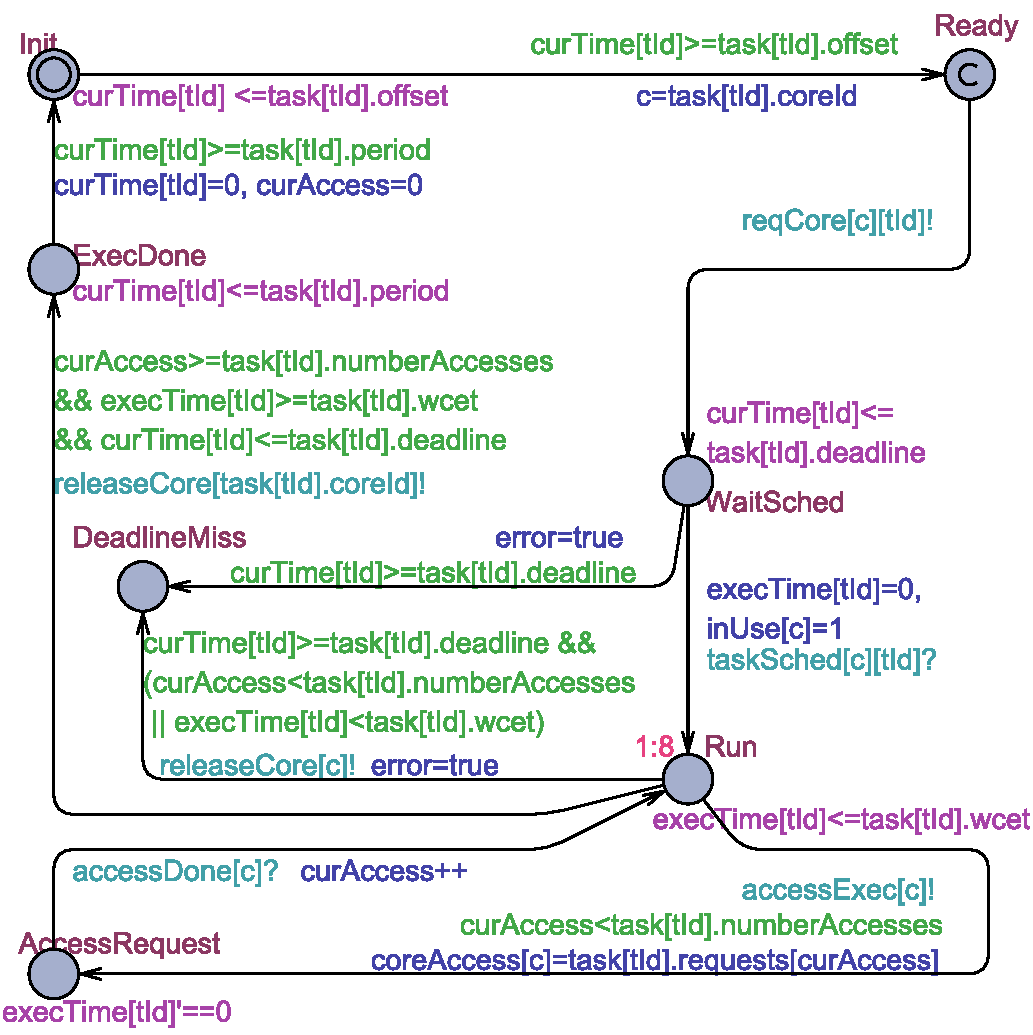
\includegraphics[scale=0.44]{Task.pdf}
\vspace{-7mm}
\end{figure}

Our Uppaal task template model is depicted in Fig.~\ref{fig:task}. To distinguish between different tasks, we associate to each task an identifier \texttt{tId} as a template parameter. The task starts at location \ft{Init} where it initializes its variables if needed, during the offset time. Once the offset expires, the task moves to location \ft{Ready} to request the core (\emph{c}) it is mapped to, through a synchronization with the core scheduler on channel \texttt{reqCore}. The task waits to be scheduled at location \ft{WaitSched} unless the deadline is reached by which it moves to location \ft{DeadlineMiss} and updates a global variable \emph{error} to true. Once a task is scheduled it updates the status of the corresponding core \emph{inUse[c]=1}, and moves to location \ft{Run} to execute. The status update of variable \emph{inUse[c]} leads the clock accumulating the core utilization to resume. During its execution (\emph{WCET}), a task non-deterministically triggers access requests to L2 and DRAM. For each access request, the task moves to location \ft{AccessRequest} and waits until the access request is satisfied upon which it moves back to location \ft{Run}. One can remark that, when a task is requesting and waiting for data the clock measuring \emph{WCET} is stopped (\emph{execTime[tId]'==0}) so that only the effective execution at \ft{Run} consumes \emph{WCET}. This is implemented in Uppaal by assigning rate 0 to the derivative of \emph{execTime[tId]}. Such a clock resumes at \ft{Run}. From \ft{Run}, the task joins either \ft{ExecDone}, if the execution \emph{WCET} and accesses to L2 and DRAM ($\emph{numberAccesses=WCRA}_c^r\emph{+WCRA}_c^w \emph{+WCRA}_m^r\emph{+WCRA}_m^w$) are completed before deadline, or it moves to location \ft{DeadlineMiss} in case the execution or access requests are not achieved before deadline. Once the period expires, at location \ft{ExecDone}, the task moves to \ft{Init} to start a new period. The task template can be instantiated for different tasks by just providing the aforementioned parameters.%, specified in the aforementioned definition.
  

\subsection{Platform Model}
A platform is given by a set of processing elements {\cal PE}, sharing a cache level L2 and DRAM memory, and schedulers to manage the access to L2 and DRAM. Each processing element PE is given by a computation resource (core), a local cache memory and a scheduler to dispatch tasks to run on that core. The access time for local caches may vary from one PE to another. In fact, such a number corresponds to a cache hit. In case of a cache miss, extra delay will result from accessing the shared memory. %Moreover, we consider the time duration for an effective access (from grant to completion) to a shared memory as a platform parameter. 

\subsubsection{Modeling of Processing Elements}
A processing element PE is given by $\langle C, sched, H\rangle$ where $C$ is a core, $sched$ is the scheduling policy (core scheduler) adopted and $H$ is the local cache that we abstract using its access time $LocalCacheTime$. The core model is depicted in Fig.~\ref{fig:core}.  

\begin{figure}
\centering
\caption{Core template model}
\label{fig:core}
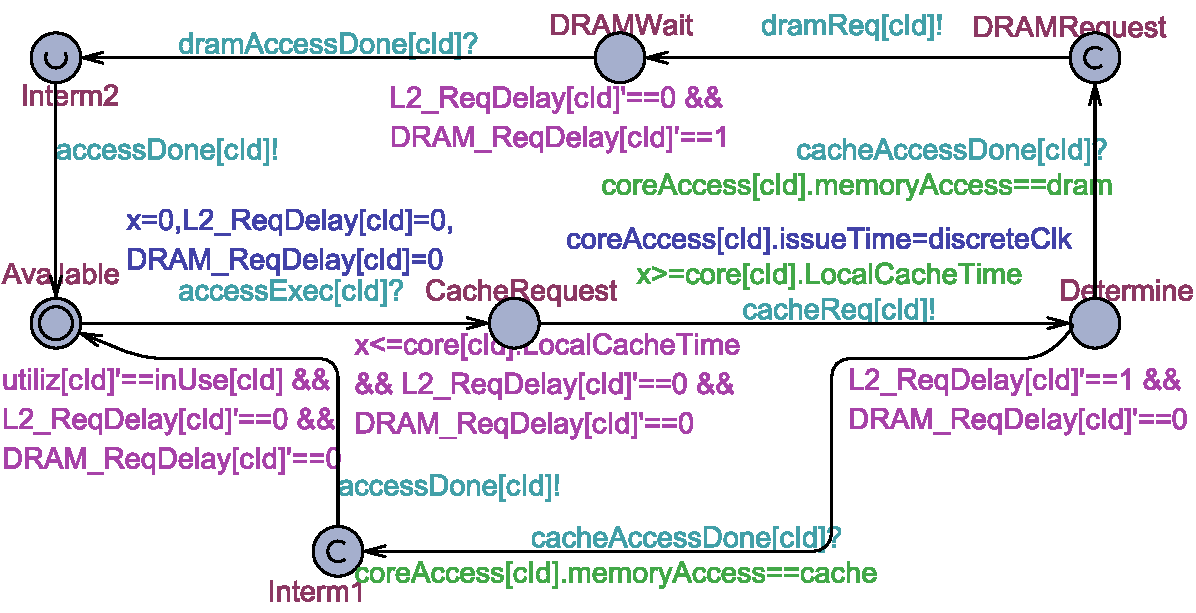
\includegraphics[scale=0.41]{Core.pdf}
\vspace{-3mm}
\end{figure}

Similarly to tasks, we assign to each core an identifier \texttt{cId} as a parameter to distinguish between the different platform cores. The core model is initially at location \ft{Available} waiting for ready tasks. Through an allocation, the core model does not move from \ft{Available} but the clock measuring its utilization \emph{utiliz[cId]} starts counting (\emph{utiliz[cId]'==inUse[cId]}). Such a clock can stop and resume according to the core status \emph{inUse[cId]} manipulated at task level. Upon an access request to a shared memory (\emph{accessExec[cId]?}), the core moves to location \ft{CacheRequest} where it waits for the expiry of the local cache access time \emph{LocalCacheTime} before performing the access request to the shared cache L2 and joins location \ft{Determine}. The core updates the request issue time with the current time instant \emph{issueTime=discreteClk}. At that location, the clock measuring the core delay for the current access to L2 starts (\emph{L2\_ReqDelay[cId]'==1}). 
Once the access to L2 hits (\emph{memoryAccess==cache}) and terminates, the clock \emph{L2\_ReqDelay[cId]} gets preempted (\emph{L2\_ReqDelay[cId]'==0}) and the core moves back immediately to location \ft{Available} to continue executing the assigned task. Otherwise, once the L2 access terminates and misses (\emph{memoryAccess==dram}) the core requests access to DRAM and joins immediately the location \ft{DRAMWait}, whereby the clock measuring the core delay for the current access request is released (\emph{DRAM\_ReqDelay[cId]'==1}). Once the current access is completed, clock \emph{DRAM\_ReqDelay[cId]} gets preempted while holding the measured delay. Upon the release of new access requests, from location \ft{Available}, clocks \emph{L2\_ReqDelay[cId]} and \emph{DRAM\_ReqDelay[cId]} are reset. 
  
The core blocking time on an access request (at locations \ft{Determine} and \ft{DRAMWait}) depends on the access nature. If it is a write action, the core will immediately be unlocked by the scheduler of the targeted memory, otherwise the core stalls until the read access finishes. Further details regarding how to handle read and write accesses will be provided in the description of L2 and DRAM schedulers.    

The core needs to notify the running task when the current access request is done, i.e. once the core itself is notified by DRAM or L2 (according to the access pattern), so that the task moves back as well from location \ft{AccessRequest} to \ft{Run} and accounts a granted access (\emph{curAccess++}). As it is not possible to entitle a transition with two synchronization events in Uppaal, we introduce two intermediate locations \ft{Interm1} and \ft{Interm2}. Thus, we create a sequence of 2 synchronizations without any delay between them. We use \textit{urgentness} and \textit{committedness} of Uppaal to enforce time to not elapse at a given location (locations marked with \texttt{U} and \texttt{C}).

\begin{figure}
\centering
\vspace{-2mm}
\caption{Scheduler template model}
\label{fig:sched}
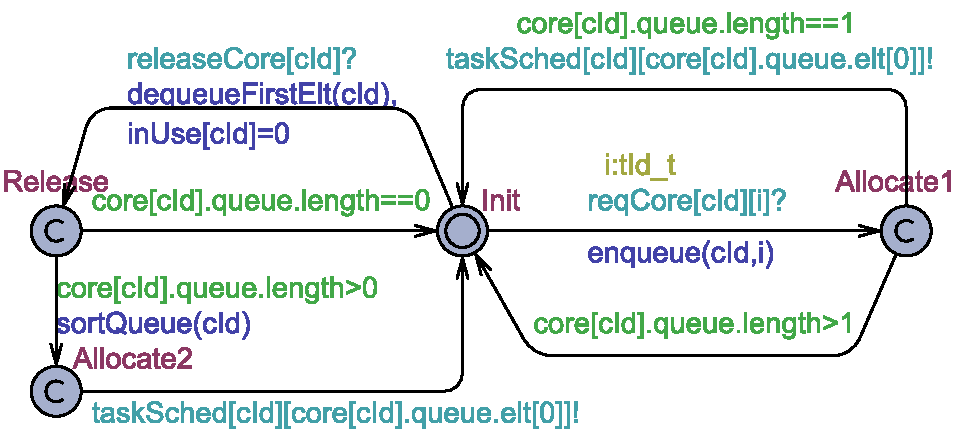
\includegraphics[scale=0.46]{Scheduler.pdf}
\vspace{-7mm}
\end{figure}

 Fig.~\ref{fig:sched} depicts the core scheduler model. Initially at location \ft{Init} waiting for a ready task request, the core moves to location \ft{Allocate1} while queuing the identifier of the requesting task. If the core queue contains only one element (\emph{queue.length==1}), which is the identifier of the newly added task, that task will immediately be scheduled otherwise the scheduler just moves back to \ft{Init}. Once the core is released by the current running task, through a signal on channel \emph{releaseCore}, the scheduler moves to \ft{Release} while removing the first element of the queue. If the queue is still not empty, the scheduler calls the adopted scheduling policy \emph{sortQueue()} of core $cId$ to sort the queue and moves to location \ft{Allocate2}, whereafter it schedules the task corresponding to the new first element in the queue. Function \emph{sortQueue(cId)} refers to the scheduling policy of core \emph{cId}, which is a core parameter in our model and can be FIFO, FPS, EDF or memory-centric.   
   
\subsubsection{Modeling of Shared Memories}
This section describes the modeling of L2 cache, DRAM and their schedulers.  
A DRAM=$\langle \emph{DRAMStruct, DRAMSched, DRAMAccessTime}\rangle$ is given by a structure \emph{DRAMStruct} (Fig.~\ref{fig:dram}), a scheduler \emph{DRAMSched} (Fig.~\ref{fig:dramsched}) and the time duration for an effective access \emph{DRAMAccessTime}. The DRAM access time simulates the duration of fetching data from a physical address in DRAM once the access is scheduled. This is in fact to enable our abstraction of the DRAM internal architecture to capture the delay for accessing a DRAM bank/row. Our DRAM model can be viewed as a one-bank memory that is shared between all cores, but it can easily be extended for several banks by just duplicating the DRAM structure and assigns each to one core only \cite{Heechul2015}. Moreover, we assume that the instantiation of our L2 and DRAM models satisfies the JEDEC standard \cite{Jedec}, which dictates the operation and timing constraints of memory devices such latency, opening and closing durations of banks.

%We omit specifying the size of DRAM neither the size of the cache space assigned to each application. The reason behind that is that the impact of these characteristics on the interference is already captured by $WCRA_m$ and $WCRA_c$, however the size of such spaces is a primordial element in the calculation of WCRAs and cache miss ratio.

The DRAM structure model (Fig.~\ref{fig:dram}) is initially waiting at location \ft{Idle} for an access request, either read or write. DRAM can be allocated, by its scheduler, to a given core \emph{i} performing a read request \emph{DRAMReqR[i]?} and moves to location \ft{Read}. Similarly, DRAM can be targeted with a write request \emph{DRAMReqW?}.

One can see that for write access requests the identifier of the involved core is missing. This is because write requests are not blocking, thus no need to keep track of which core needs to be unlocked once the access is done. At locations \ft{Read} and \ft{Write}, the DRAM waits for the expiry of the access time \emph{$DRAMAccessTime$} then moves to location \ft{Done}. From \ft{Read}, once the access time expires the DRAM unlocks the involved core through a synchronization \emph{dramAccessDone[currentCore]!}, whereas from location \ft{Write} no unlock action is needed. From \ft{Done}, DRAM notifies its scheduler that the current access is done, so that other requests can be performed.  
  
%Upon a read request, the DRAM is allocated to the requesting core and moves to location \ft{Access} where it waits for the effective access time $DRAMAccessTime$ to expire. Once such a duration expires, the DRAM notifies the requesting core so that it resumes its regular execution ($dramAccessDone!$). The DRAM notifies its scheduler as well that it becomes available to satisfy other potential requests ($releaseDRAM!$).   

\begin{figure}[ht]
\centering
\vspace{-3mm}
\caption{DRAM template model}
\label{fig:dram}
\vspace{-2mm}
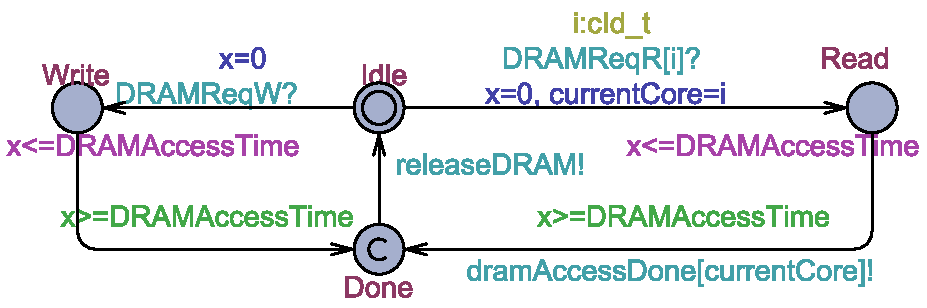
\includegraphics[scale=0.53]{DRAMMemory.pdf}
\vspace{-3mm}
\end{figure}

We adopt the FR-FCFS policy to arbitrate accesses to DRAM. We assume that row opening and reload actions are instantaneous, so that we do not need to consider any preference based on the \textit{already open row} policy \cite{Kim14}. This leads us to consider the attribute \emph{issueTime} of each request as a \textit{readiness}. Hence, we characterize each request to DRAM with another new attribute \emph{arrivalT}, besides to \emph{issueTime}. In fact, \emph{issueTime} stores the time instant when the request is issued, whereas \emph{arrivalT} stores the instant when the request reaches the corresponding bank queue. Thus, we compare requests first based on their issue times (readiness) where an earlier request has priority over later ones. If requests have the same issue time, then the request having an earlier \emph{arrivalT} has priority over requests having later \emph{arrivalT}. 

The DRAM scheduler is depicted in Fig.~\ref{fig:dramsched}. Initially at location \ft{Init}, upon the receive of an access request \emph{dramReq[i]?} from any core \emph{i} the DRAM scheduler inserts such a request together with the identifier of the requesting core into the queue and moves to location \ft{Allocate1}. If such a request is a write (\emph{rwAction==Write}), the requesting core will immediately be unlocked (\emph{dramAccessDone[l]!}) as location is committed \ft{Allocate1}. Moreover, the write request is alone in the queue (\emph{queue.length==1}) it will immediately be scheduled at location \ft{Unlocked}.
In case of a read request (\emph{rwAction==Read}), the DRAM scheduler does not unlock the requesting core after queuing the request, but it just schedules the access (\emph{DRAMReqR[DRAM.queue.elt[0].core]!}) if the current request is alone in the queue. In all of the four scenarios, the scheduler moves back to location \ft{Init}.

Once an access request is performed, the scheduler is notified by the DRAM through a synchronization event \emph{releaseDRAM?} and moves to \ft{Release} while removing the head of the queue. If the queue is still not empty, the scheduler calls the algorithm FR-FCFS to sort the queue as other requests might join during the execution of the last access. At location \ft{Allocate2}, the scheduler schedules the request in the first element of the queue \emph{queue.elt[0]} using the appropriate channel (\emph{DRAMReqR} or \emph{DRAMReqW}) according to the request nature; read or write.  

\begin{figure}[htb]
\centering
\vspace{-3mm}
\caption{DRAM scheduler model}
\label{fig:dramsched}
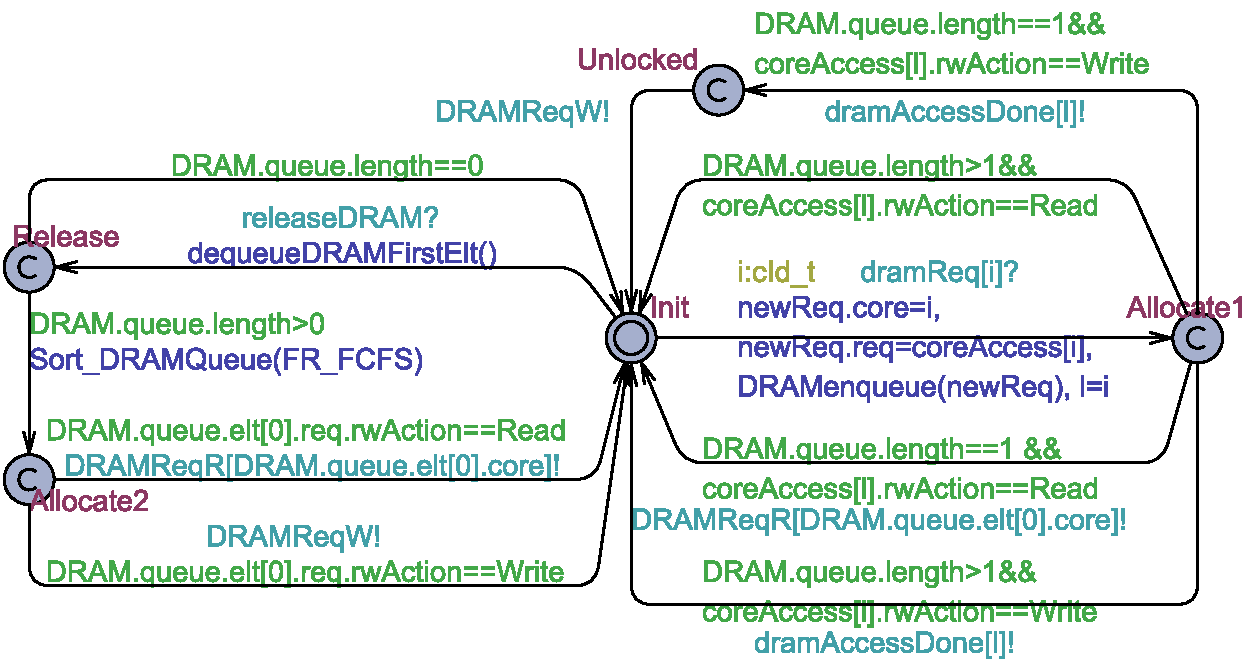
\includegraphics[scale=0.41]{DRAMScheduler.pdf}
\vspace{-3mm}
\end{figure}

Due to space limitations, we omit describing the shared cache L2 and its scheduler. In essence, L2 has the same elements as DRAM , except that it uses a separate queue to store its requests. Similarly, L2 scheduler has the same behavior as that of DRAM but it operates on the L2 queue using the cache coloring policy. However, since we do not consider the internal pages of L2, the coloring policy adopted in our framework behaves in similar way to FCFS policy.

Finally, a platform \emph{P} is given by \begin{footnotesize}\emph{$\langle \langle PE_1, .., PE_m \rangle, DRAM, L2\rangle$}\end{footnotesize}. One can see that updating the specification of one platform ingredient does not necessarily affect the others. %In case a new memory connector needs to be used instead (for example FCFS), we simply replace the bus $B$ with the new connector. 

\subsection{System Model}
In order to make our framework flexible, the application and platform are specified separately then mapped together. A system model $S$ is given by an application \emph{$AP=\{T_1,..,T_n\}$}, a platform \emph{$P=\langle {\cal PE}, DRAM, L2\rangle$} and a mapping \emph{$M:AP \rightarrow {\cal PE}$} assigning each task to a processing element \emph{$PE_i \in {\cal PE}$}. %A task can only be assigned to one core, however a core can serve different tasks.




\section{Performance Analysis}
\label{sec:analysis}
This section gives a technical description of the performance and schedulability analysis, as well as a discussion about how the  performance analysis outcomes are interpreted and compared. 

\subsection{Schedulability Analysis}
In our framework, the system schedulability is analyzed as a reachability property using symbolic model checking \cite{Facs2013}. Following our task model, whenever a process misses its deadline it joins immediately the location \ft{DeadlineMiss} (by which the global variable \emph{error} is updated to true). Thus, the schedulability analysis process simply checks whether any task can reach its own \ft{DeadlineMiss} location. Technically, to quantify on all tasks regardless of their identifiers we use the following CTL query supported by Uppaal: \[ \forall []~ \emph{!error}~~~(1)
\]

\subsection{Memory Interference Analysis}
To analyze the delays of access requests performed by a given core, we need to run the execution simulation several times ($X$) each of which lasts for $Y$ time units. The simulation time $Y$ should be greater than the least common multiplier of periods of the tasks mapped to such a core. In fact, the larger $X$ and $Y$ are the more accurate the results will be. To display the average delays of a core $C$, to access L2 and DRAM respectively, in terms of probability distributions we use the following SMC queries: 
\[\begin{array}{ll} E[clk<=Y;X](max:\emph{L2\_ReqDelay}[C]) & (2) \\
                    E[clk<=Y;X](max:\emph{DRAM\_ReqDelay}[C]) & (3) \end{array}
\]

Fig.~\ref{fig:delays} shows the probability distributions of the request delays to L2 and DRAM of a core $C$ where $X=10^3$ and $Y=10^4$. $C$ runs in parallel with another core, each of which serves 2 tasks. Values 2.96 and 4 are the most likely L2 and DRAM access delays respectively because they have the highest probabilities. 

\begin{figure}[ht!]
\centering
\vspace{-5mm}
\caption{L2 and DRAM Request delays.}
\label{fig:delays}
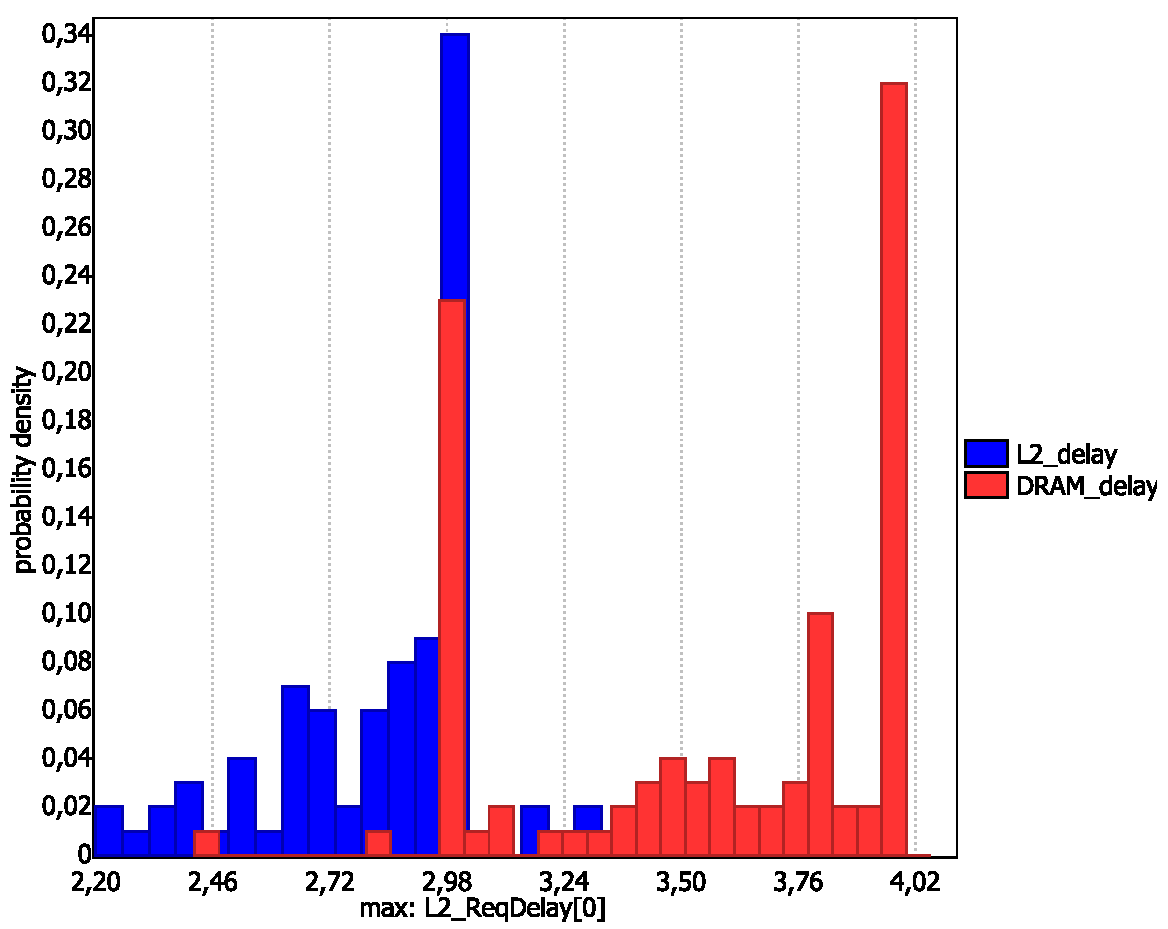
\includegraphics[width=87mm,height=47mm]{Both-delays.pdf}
\end{figure}

																	
\subsection{Utilization Analysis}
To analyze the utilization of cores, we need to run the execution simulation several times ($X$) each of which lasts for $Y$ time units. We accumulate for each simulation the core utilization time via clock \emph{utiliz[cId]}, we consider then the maximum value using the following SMC query:
\[ \begin{array}{ll} \emph{simulate}~ X~ [<=Y]~ {\emph{utiliz}[cId]} &(4) \end{array}\]

\begin{figure}[ht!]
\centering
\vspace{-5mm}
\caption{Simulation of cores utilization.}
\label{fig:core0_utiliz_simul}
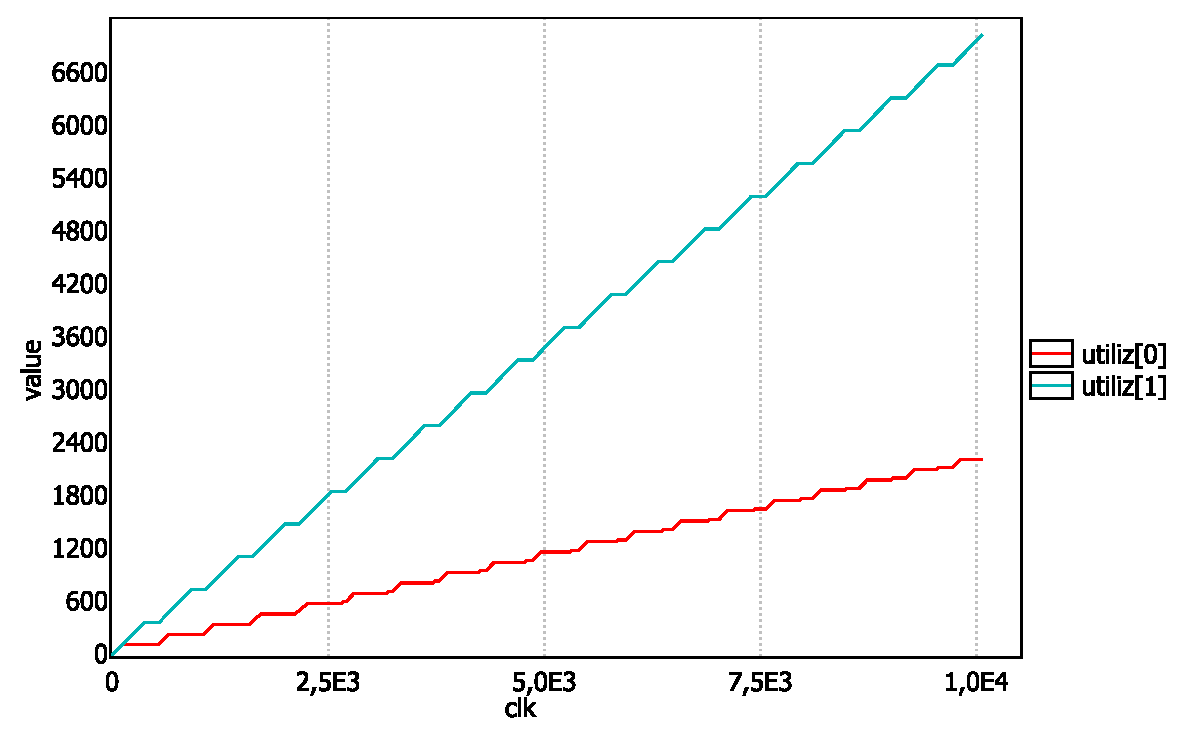
\includegraphics[width=77mm,height=39mm]{Core0_utiliz_Simulation2.eps}
\vspace{-4mm}
\end{figure}

The utilization degree of a given core is then obtained by dividing the accumulated utilization time over the total simulation time $Y$. Fig.~\ref{fig:core0_utiliz_simul} shows the average accumulated utilization time of 2 individual cores ($C_0$ and $C_1$) for 1000 simulations. Each simulation runs for 10000 clock ticks (query (4)). Thus, the utilization of core $C_0$ is $2223/10^4*100=22.2\%$. %The cores utilization can be generated as well in terms of a probability distribution %Similarly, the maximum utilization of a given core can be generated in terms of a probability distribution using the following query: \[\begin{array}{ll} E[clk<=Y;X](max:utiliz[cId]) & (5) \end{array}\]

The fact that read requests are blocking, they contribute majorly in the cores utilization by making cores stalling.  
On the other hand write accesses are not blocking and have a less important impact on the utilization, even though write accesses make the waiting queue longer, which some how might delay other read accesses.

\subsection{Performance Comparison}
We use the multi-objective Pareto frontier to compare the performance of system configurations having different scheduling policies. We emphasize that we compare different configurations of the \textit{same} system, where only scheduling policies vary from a configuration to another. Hence, our framework cannot be used to compare unrelated systems. To perform comparison, one can keep varying scheduling policies, while schedulability and functional requirements are satisfied, until better performance is achieved.   

 

 





\section{Case Study}
\label{sec:casestudy}
To illustrate the applicability of our performance-driven scheduling framework, we consider two case studies: a Mission Control Computer avionic system MCC \cite{Locke91} and an Autonomous Vehicle Component AVC \cite{HyoseungData14}. MCC is CPU-intensive whereas SVC is memory-intensive. We analyze and compare the performance achieved by each case study when running core-centric and memory centric. The diversity of the case studies gives a practical experience on what is the appropriate scheduling policy to be used for each application category to achieve high performance. 

%***AS WCRAs are not provided in the original case studies, we calculate them by dividing the time spent by each task to fetch data over the average duration for one access. Moreover, as the numbers of access requests to shared cache and DRAM are not explicitly distinguishable in both case studies, we rely on the analysis results obtained by Ye \textit{et al.} \cite{Ye2014} using the cache coloring policy, where only 22.2\% of the access requests hit the L2 cache while 77.8\% of the requests need to access to DRAM. 

The time durations for effective accesses to L2 ($L2AccessTime$) and DRAM ($DRAMAccessTime$) are $1/10^3$ and $1/10^2$ milliseconds respectively. Moreover, all time units are given in milliseconds. 

\subsection{MCC Example}
MCC is a partial specification for a hypothetical avionics mission control computer system dedicated to combat and attack
aircrafts. The application we consider is a composition of 13 tasks having the characteristics shown in Table~\ref{tab:taskset1}, where \emph{WCRA}$_c$ and \emph{WCRA}$_m$ are given in terms of (reads; writes). Tasks are grouped in 4 components \{\emph{Display}=($T_1,T_2,T_3,T_4,T_5$), \emph{Radar}=($T_6,T_7$), \emph{{NAV}}=($T_8,T_9,T_{10}$), \emph{Weapon}=($T_{11},T_{12},T_{13}$)\} running each on one core \cite{Boudjadar15}. 

****provide wcra for each task***
\begin{table}
\centering
\caption{Attributes of the MCC tasks}
\label{tab:taskset1}
\vspace{1mm}
\begin{tabular}{|l|l|l|l|l|l|l|}
\hline
Task & Prd & Offset & WCET & WCRA$_c$ & WCRA$_m$ & Dln  \\
\hline  \hline
$T_1$ & 200 & 0 & 3 & (X; X) & (Y; Y) & 200 \\
\hline 
$T_2$ & 200 & 0 & 1 & (X; X) & (Y; Y) & 200 \\
\hline 
$T_3$ & 80 & 0 & 2 &(X; X) & (Y; Y) & 80 \\
\hline 
$T_4$ & 80 & 0 & 9 &(X; X) & (Y; Y) & 80 \\
\hline
$T_5$ & 200 & 0 & 1 &(X; X) & (Y; Y) & 200 \\
\hline
$T_6$ & 50 & 0 & 5 & (X; X) & (Y; Y) & 50 \\
\hline 
$T_7$ & 25 & 0 & 2 & (X; X) & (Y; Y) & 25 \\
\hline 
$T_8$ & 59 & 0 & 8 &(X; X) & (Y; Y) & 59 \\
\hline 
$T_9$ & 200 & 0 & 3 &(X; X) & (Y; Y) & 200 \\
\hline
$T_{10}$ & 1000 & 0 & 1 &(X; X) & (Y; Y) & 1000 \\
\hline
$T_{11}$ & 200 & 0 & 1 &(X; X) & (Y; Y) & 200 \\
\hline
$T_{12}$ & 200 & 0 & 3 &(X; X) & (Y; Y) & 200 \\
\hline
$T_{13}$ & 50 & 0 & 3 & (X; X) & (Y; Y) & 50 \\
\hline 
$T_{14}$ & 200 & 0 & 3 & (X; X) & (Y; Y) & 200 \\
\hline 
$T_{15}$ & 50 & 0 & 3 &(X; X) & (Y; Y) & 50 \\
\hline
\end{tabular}
\vspace{-2mm}
\end{table}

***Analysis results

\subsection{AVC Example}
AVC is a component of an autonomous vehicle system \cite{HyoseungData14}. The task functions are obtained from the PARSEC benchmark suite \cite{Bienia2008} and used to capture different components of complex real-time embedded applications such as sensor fusion and computer vision in an autonomous vehicle system.


Essentially, the application consists of 4 periodic tasks $T_1$ (StreamCluster), $T_2$ (Ferret), $T_3$ (Canneal) and $T_4$ (FluidAnimation) running on 2 identical cores ($C_0$ and $C_1$) sharing L2 and DRAM. $T_1$ and $T_2$ are assigned to $C_0$, whereas $T_3$ and $T_4$ execute on $C_1$. The characteristics of the task set are shown in Table~\ref{tab:taskset}.     
 \begin{table}
\centering
\caption{Attributes of the AVC tasks}
\label{tab:taskset}
\vspace{1mm}
\begin{tabular}{|l|l|l|l|l|l|l|}
\hline
Task & Prd & Offset & WCET & WCRA$_c$ & WCRA$_m$ & Dln  \\
\hline  \hline
$T_1$ & 400 & 0 & 120 & (40; 0) & (110; 10) & 400 \\
\hline 
$T_2$ & 1200 & 0 & 130 & (60; 60) & (136; 273) & 1200 \\
\hline 
$T_3$ & 1800 & 0 & 500 &(134; 266) &(705; 705) & 1800 \\
\hline 
$T_4$ & 6000 & 0 & 440 &(314; 626) &(1828; 1462) & 6000 \\
\hline
\end{tabular}
\vspace{-2mm}
\end{table}

***Analysis results

%
%The platform description is given in Table~\ref{tab:platform}, where $H$ is the access time for the core local cache. 
Both cores run EDF schedulers (core-centric), while the access time to the local cache lasts for $1/10^3$ millisecond. 

%\begin{table}
%\centering
%\caption{Platform description and mapping}
%\label{tab:platform}
%\vspace{3mm}
%\begin{tabular}{|l|l|l|l|}
%\hline
%Core & Sched policy& H & Mapped tasks \\
%\hline
%$C_1$ & EDF & 1/$10^3$& $T_1, T_2$ \\
%\hline
%$C_2$ & EDF & 1/$10^3$& $T_3, T_4$ \\
%\hline
%\end{tabular}
%\end{table}

Each of the statistical analysis results of the case study has been calculated from 1000 simulations. Each simulation experiment runs for 1 million clock ticks. The accumulated utilization times of cores $C_0$ and $C_1$ are depicted in Fig.~\ref{fig:cores_utiliz}. During 1 million time units, cores accumulate 419983 and 360350 respectively. Thus, the average utilization of $C_0$ is $42\%$ and the average utilization of $C_1$ is $36\%$. Schedulability analysis shows that the system is schedulable. 

Add analysis of average delay to access L2 and DRAM *****

Second alternative: when using a memory-centric scheduling policy****

%Since the system requirements are met and the core workloads are modest and relatively comparable, there is no need to migrate any task. The longest analysis time spent by Uppaal is 3426.7 seconds. The performance and analysis results from the case study are encouraging and suggest that the framework might scale to larger systems.

%\begin{figure}[ht!]
%\centering
%\vspace{-3mm}
%\caption{Accumulated cores utilization.}
%\label{fig:cores_utiliz}
%\includegraphics[width=80mm,height=48mm]{utiliz_Result_Simulation2++.png}
%\end{figure}   

**case study2***


****Discussion of the performance results and how one would choose the appropriate scheduling policy.


\section{conclusion}
\label{sec:conclusion}

%This paper introduces a model-based framework for schedulability and interference sensitive WCET analysis. The framework captures both the multicore platform and system application given in terms of periodic non preemptive tasks. Our framework is realized using timed automata and stopwatch clocks of Uppaal, while the analysis is performed using both statistical and symbolic model checking techniques. In case of non-schedulability, we provide a technique to analyze the cores utilization and study the impact of tasks migration with the goal to find potential mappings with which the system becomes schedulable.
***Summary of the paper

As future work, we plan to compare the performance results obtained using our framework with the state of the art tools \cite{6280389,10.1109/MS.2005.102}. We intend also to incorporate detailed architectures of L2 and DRAM, consider other factors in the derivation of configurations such as task-to-core mapping where we reallocate tasks to cores differently and the use of other performance metrics such as energy consumption. 


\bibliographystyle{abbrv}
\bibliography{references}

%\listoftodos

\end{document}
